\documentclass[11pt,a4paper]{article}
\usepackage[T1]{fontenc}
\usepackage{graphicx}
\usepackage{amsmath,amssymb,amsthm,amsfonts}
\usepackage{geometry}\geometry{left=2.3cm,right=2.3cm,top=2.5cm,bottom=2.5cm}
\usepackage{setspace}\setstretch{1.20}
\usepackage{hyperref}\hypersetup{colorlinks=true,linkcolor=black,citecolor=black}
\usepackage{parskip,booktabs,array,xcolor,titlesec,enumitem,microtype}
\microtypesetup{expansion=false}
\titleformat{\section}{\large\bfseries}{}{0em}{}[\titlerule]
\titlespacing{\section}{0pt}{14pt}{6pt}
\titleformat{\subsection}{\normalsize\bfseries}{\thesubsection\;}{0em}{}
\newtheorem{remark}{Remark}
\begin{document}
\begin{center}
{\LARGE\bfseries Numerical Protocol}\\[0.3cm]
{\large Log-Volatility Roughness Evaluation\\
under the Log-Normal SV DGP with fBM}\\[0.2cm]
{\normalsize Othmane Zarhali}
\end{center}
\vspace{0.15cm}\noindent\rule{\textwidth}{0.8pt}
\begin{abstract}

We evaluate the roughness of $\log V_t$ under the log-normal Stochastic volatility DGP:

\begin{enumerate}
    \item \textbf{Data generation.} Simulate the log-normal stochastic volatility process
    \[
    \sigma_t=\sigma_0\exp\!\left(\lambda B^H(t)-\frac{\lambda^2}{2}t^{2H}\right),
    \]
    where the fractional Brownian motion $B^H$ is generated by Cholesky decomposition of its covariance matrix.

    \item \textbf{Reference properties.} Use the analytical properties of the DGP as the benchmark:
    \begin{itemize}
        \item the variogram has an exact slope equal to $2H$;
        \item the log volatility process is monofractal, satisfying
        \[
        \zeta(q)=qH,\qquad
        H(q)\equiv H,\qquad
        \mu(q)\equiv0.
        \]
    \end{itemize}

    \item \textbf{Model calibration.} Calibrate three competing models to the complete stylised-fact profile of the DGP:
    \begin{itemize}
        \item ESN A2-981003, using its current optimal architecture
        \[
        (N_r,N_z)=(96,12),
        \]
        and the smooth Gaussian-kernel score;
        \item QRH;
        \item PDV-GL.
    \end{itemize}

    \item \textbf{Model evaluation.} Assess each calibrated model by comparing its reproduction of the DGP roughness through three complementary diagnostics:
    \begin{enumerate}
        \item OLS estimation of the Hurst exponent;
        \item linearity of the autocovariance as a function of $\tau^{2\hat H}$;
        \item estimation of the multifractal spectrum.
    \end{enumerate}
\end{enumerate}
\end{abstract}
\tableofcontents\vspace{0.4cm}
\section{DGP: Log-Normal SV with fBM}
\begin{equation}
  r_t=\sigma_t\varepsilon_t,\quad\varepsilon_t\sim\mathcal{N}(0,1),\qquad
  \sigma_t=\sigma_0\exp\!\Bigl(\lambda B^H(t)-\tfrac{\lambda^2}{2}t^{2H}\Bigr).
\end{equation}
The centring term $-\lambda^2 t^{2H}/2$ ensures $\mathbb{E}[\sigma_t]=\sigma_0$.
Analytical truth: $m_2(\tau)=4\lambda^2\tau^{2H}$, so OLS variogram slope $=2H$ exactly.
DGP is monofractal: $\zeta(q)=qH$, $H(q)\equiv H$, $\mu(q)\equiv0$.
Simulation via Cholesky of $\Sigma_{ij}=\tfrac12(t_i^{2H}+t_j^{2H}-|t_i-t_j|^{2H})$, cached.
Parameter grid available: $H\in\{0.05,0.10,0.40\}$, $\lambda\in\{0.5,1.0,2.0\}$; this
note reports the rough-target subset $H\in\{0.05,0.10\}$ at $\lambda=1.0$.
\section{Models}
All three models use Gaussian Brownian innovations.
\subsection{ESN A2-981003 (current optimal architecture)}
7 shared hyperparameters, with $N_r=96,N_z=12$.
\texttt{rough\_scale}, the $z$-readout profile ($\texttt{zr\_lo},
\texttt{zr\_hi}$), and the symmetric quadratic matrix coefficients
$(m_1,m_2)$ are calibrated per $(H,\lambda)$ cell, not part of this
fixed table (see \S3's Calibration table for their per-cell values).
\begin{table}[H]
\centering
\caption{The 7 shared hyperparameters of the optimal architecture.}
\begin{tabular}{@{}lr@{}}
\toprule
Hyperparameter & Value \\
\midrule
$N_r$ & 96 \\
$N_z$ & 12 \\
\texttt{z\_strength} & 0.1929 \\
\texttt{even\_strength} & 2.2291 \\
\texttt{linear\_strength} & 0.1930 \\
\texttt{gamma\_norm} & 0.9651 \\
\texttt{local\_z\_strength} & 0.0476 \\
\texttt{zz\_scale} & 0.0397 \\
\texttt{sign\_prob\_neg} & 0.2219 \\
\texttt{rough\_orientation} & $-1.0$ (fixed) \\
\bottomrule
\end{tabular}
\end{table}
A single $\varepsilon_t\sim\mathcal{N}(0,1)$ drives both the return and
the reservoir. $H$, the $r$-layer rate window
$[\lambda_{\rm lo},\lambda_{\rm hi}]$, and the $z$-layer rate window
$[a_{\rm lo},a_{\rm hi}]$ are \textbf{calibrated per $(H,\lambda)$ DGP
cell} (\S3) -- they are not part of the shared architecture above.
$H_{\rm ESN}$ (the reservoir's own memory-kernel exponent) is a
different object from the DGP's Hurst parameter $H_{\rm DGP}$; the
inner loop searches over $H_{\rm ESN}$ so the simulated $\hat H$
matches the DGP's target, and the two need not coincide.
\subsection{QRH}
Bourgey \& Gatheral (2026): $V_t=Y_t^2+c$, gamma kernel, Euler-Volterra
with RL weights $w_j=\Delta t^\alpha/(\Gamma(\alpha)\alpha)[(j+1)^\alpha-j^\alpha]$,
252-step ring buffer.
\subsection{PDV-GL}
Guyon \& Lekeufack (2023): two-factor power-law kernel,
$V_t=(1-\beta)\bar V+\beta[\alpha_1 F_t(\alpha_r)+(1-\alpha_1)F_t(\alpha_v)]$,
online computation.
\section{Calibration}
Calibration minimises the full 11-term data-adaptive score $S$, with
the \textbf{smooth Gaussian-kernel} proximity:
\begin{equation}
S=\sum_k w_k\bigl(1-f_k\bigr)+5\cdot\mathrm{Stress},\qquad
f(x,c,s)=\exp\!\Bigl(-\tfrac12\bigl(\tfrac{x-c}{s}\bigr)^2\Bigr)\in(0,1],
\end{equation}
$S\geq0$, $S=0$ is a perfect match on all 11 stylised facts, $S=15.3$ is
worst-possible; minimised directly (no sign flip). The smooth kernel
provides a never-zero gradient at any distance from target, unlike a
piecewise-linear tent $\max(0,1-|x-c|/s)$, which hits exactly 0 (zero
gradient) beyond one tolerance width.

\paragraph{ESN read-out.} The ESN's volatility pre-activation combines
three calibrated channels:
\begin{equation}
\eta_t = b_0 + \rho_r\,\texttt{rough\_scale}\,(q^\top r_t)
       + \sum_{j=1}^{N_z} w_{j,z}\,z_{j,t} + r_t^\top Qr_t,
\qquad w_{j,z}=\frac{\texttt{z\_readout}_j}{\sqrt{N_z}},
\qquad Q=\frac{1}{N_r}(m_1I+m_2qq^\top),
\end{equation}
where $\texttt{z\_readout}_j=\mathrm{geomspace}(\texttt{zr\_lo},
\texttt{zr\_hi},N_z)[j]$ is a per-mode profile, and $Q$ is a genuine
\textbf{symmetric} matrix (no positive-definiteness constraint): $m_1$
scales the reservoir's isotropic energy, $m_2$ scales the squared rough
factor $(q^\top r_t)^2$ specifically. \textbf{Only 7 hyperparameters
remain shared} across all $(H,\lambda)$ cells
(\texttt{z\_strength}, \texttt{even\_strength}, \texttt{linear\_strength},
\texttt{gamma\_norm}, \texttt{local\_z\_strength}, \texttt{zz\_scale},
\texttt{sign\_prob\_neg}, plus $N_r,N_z$); \texttt{rough\_scale},
\texttt{zr\_lo}, \texttt{zr\_hi}, and $(m_1,m_2)$ are calibrated
per $(H,\lambda)$ cell, exactly as $H,\lambda_{\rm lo},\lambda_{\rm hi},
a_{\rm lo},a_{\rm hi}$ already were.

\begin{center}\renewcommand{\arraystretch}{1.3}
\begin{tabular}{@{}p{3.0cm}p{6.4cm}p{5.0cm}@{}}\toprule
Model & Parameters calibrated & Remark \\\midrule
ESN A2-981003 & $H$, $\lambda_{\rm lo}$, $\lambda_{\rm hi}$, $a_{\rm lo}$,
  $a_{\rm hi}$, $\Delta b_0$, scale $s$, \texttt{rough\_scale},
  \texttt{zr\_lo}, \texttt{zr\_hi}, $m_1$, $m_2$ &
  7 shared hyperparameters fixed; full 12-dim.\ inner-loop calibrated
  per $(H,\lambda)$ cell (11-start Nelder--Mead) \\
QRH & $H$, $\nu_{\rm vol}$, $\lambda$, $c_{\rm frac}$ & \\
PDV-GL & $\beta$, $\alpha_1$, $\alpha_r$, $\alpha_v$ & \\
\bottomrule\end{tabular}\end{center}
The ESN's inner loop uses an 11-point multi-start Nelder--Mead scheme
(rough/fast, persistent/slow, intermediate, wide-band/multiscale,
long-memory extreme, strong-amplitude, weak-amplitude,
isotropic-positive, isotropic-negative, $q$-aligned-positive, and
$q$-aligned-negative starts), keeping the best-of-eleven result.
\section{Per-Cell Calibrated Read-Out Parameters}
At $\lambda=1.0$, the ESN's calibrated \texttt{rough\_scale} and
$z$-readout profile stay in a narrow band across the two rough-target
$H$ values tested; $m_1,m_2$ are both near-zero at both cells, with no
large excursion in either quadratic coefficient at this narrower $H$
range (this contrasts with a persistent target, $H=0.40$, tested
separately, where $m_1$ calibrated to a large negative value --
consistent with the general caution that this quadratic channel is
weakly and inconsistently identified across seeds and should not be
over-interpreted from any single cell).
\begin{center}\renewcommand{\arraystretch}{1.3}
\begin{tabular}{@{}lcccccc@{}}\toprule
True $H$ & \texttt{rough\_scale} & \texttt{zr\_lo} & \texttt{zr\_hi} & $m_1$ & $m_2$ & Score $S$ \\\midrule
0.05 & 0.433 & 0.032 & 0.072 & $-0.0002$ & $-0.0002$ & 3.955 \\
0.10 & 0.410 & 0.028 & 0.061 & $0.0000$ & $0.0004$ & 4.216 \\
\bottomrule\end{tabular}\end{center}

\section{Roughness Diagnostics}
\subsection{Diagnostic 1: Hurst OLS}
$\hat H=\tfrac12\cdot\operatorname{OLS slope}$ of $\log m_2(L)$ vs $\log L$,
$L\in\{1,2,4,8,16,32,64\}$. Cross-path 95\% CI from empirical quantiles.
\begin{figure}[H]
\centering
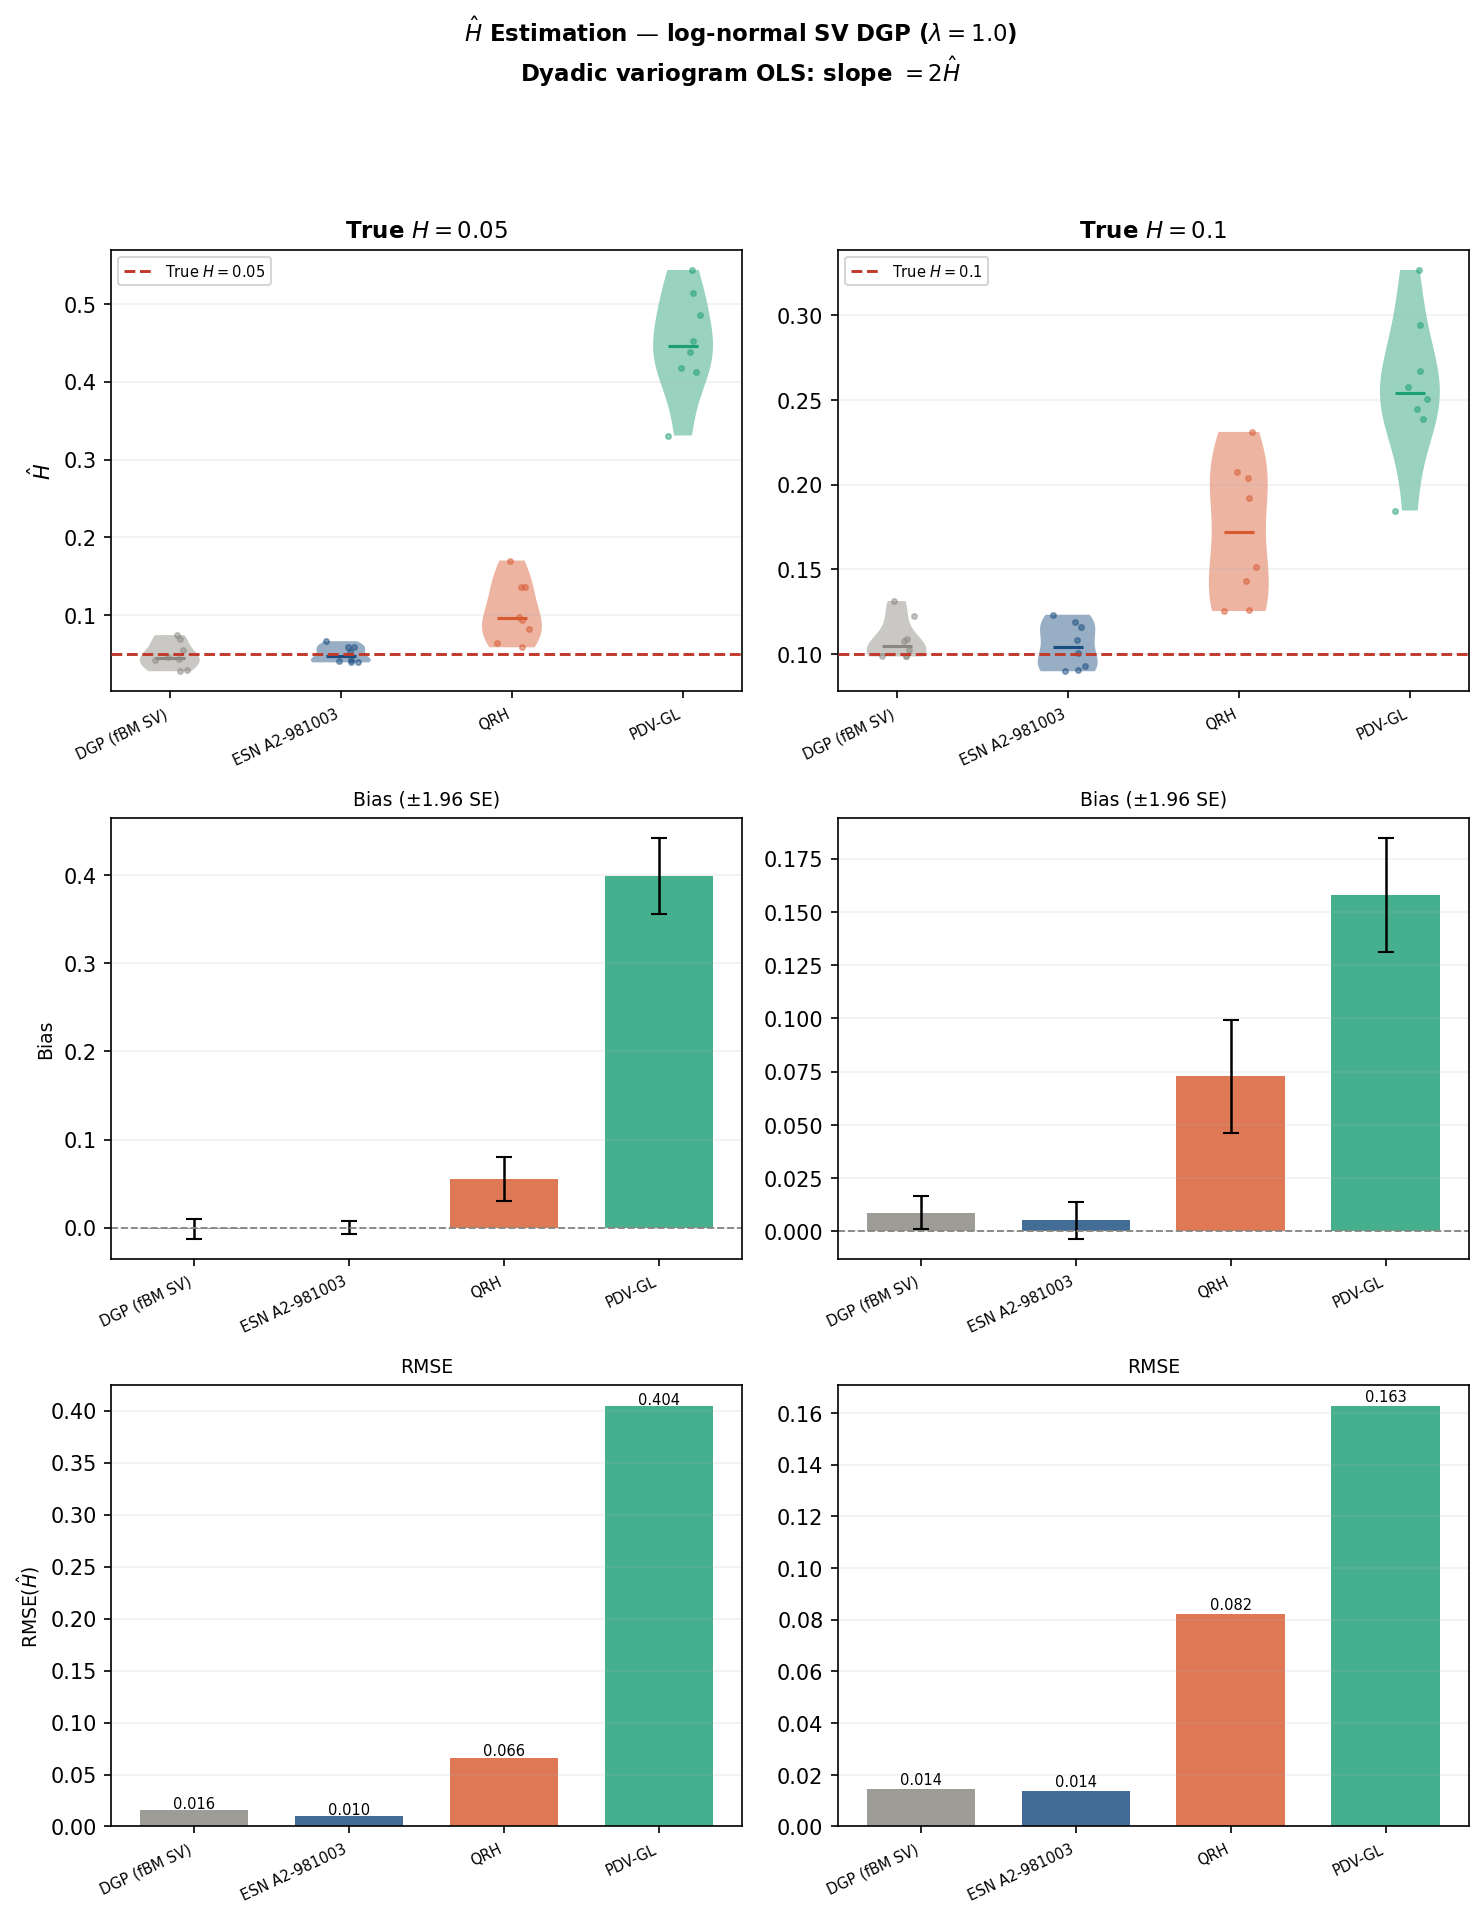
\includegraphics[width=0.95\textwidth]{roughness_h05_h10_out_hurst_lam1p0.png}
\caption{$\hat H$ estimation via the dyadic-variogram OLS slope, per model and true $H\in\{0.05,0.10\}$: violin plots of the cross-path $\hat H$ distribution (top row), bias $\pm1.96$ SE (middle row), and RMSE$(\hat H)$ (bottom row).}
\label{fig:hurst}
\end{figure}
\subsection{Diagnostic 2: ACov linearity}
OLS: $C(\tau)/C(0)=a+b\tau^{2\hat H}$. $R^2\to1$ = correct Hölder exponent.
\begin{figure}[H]
\centering
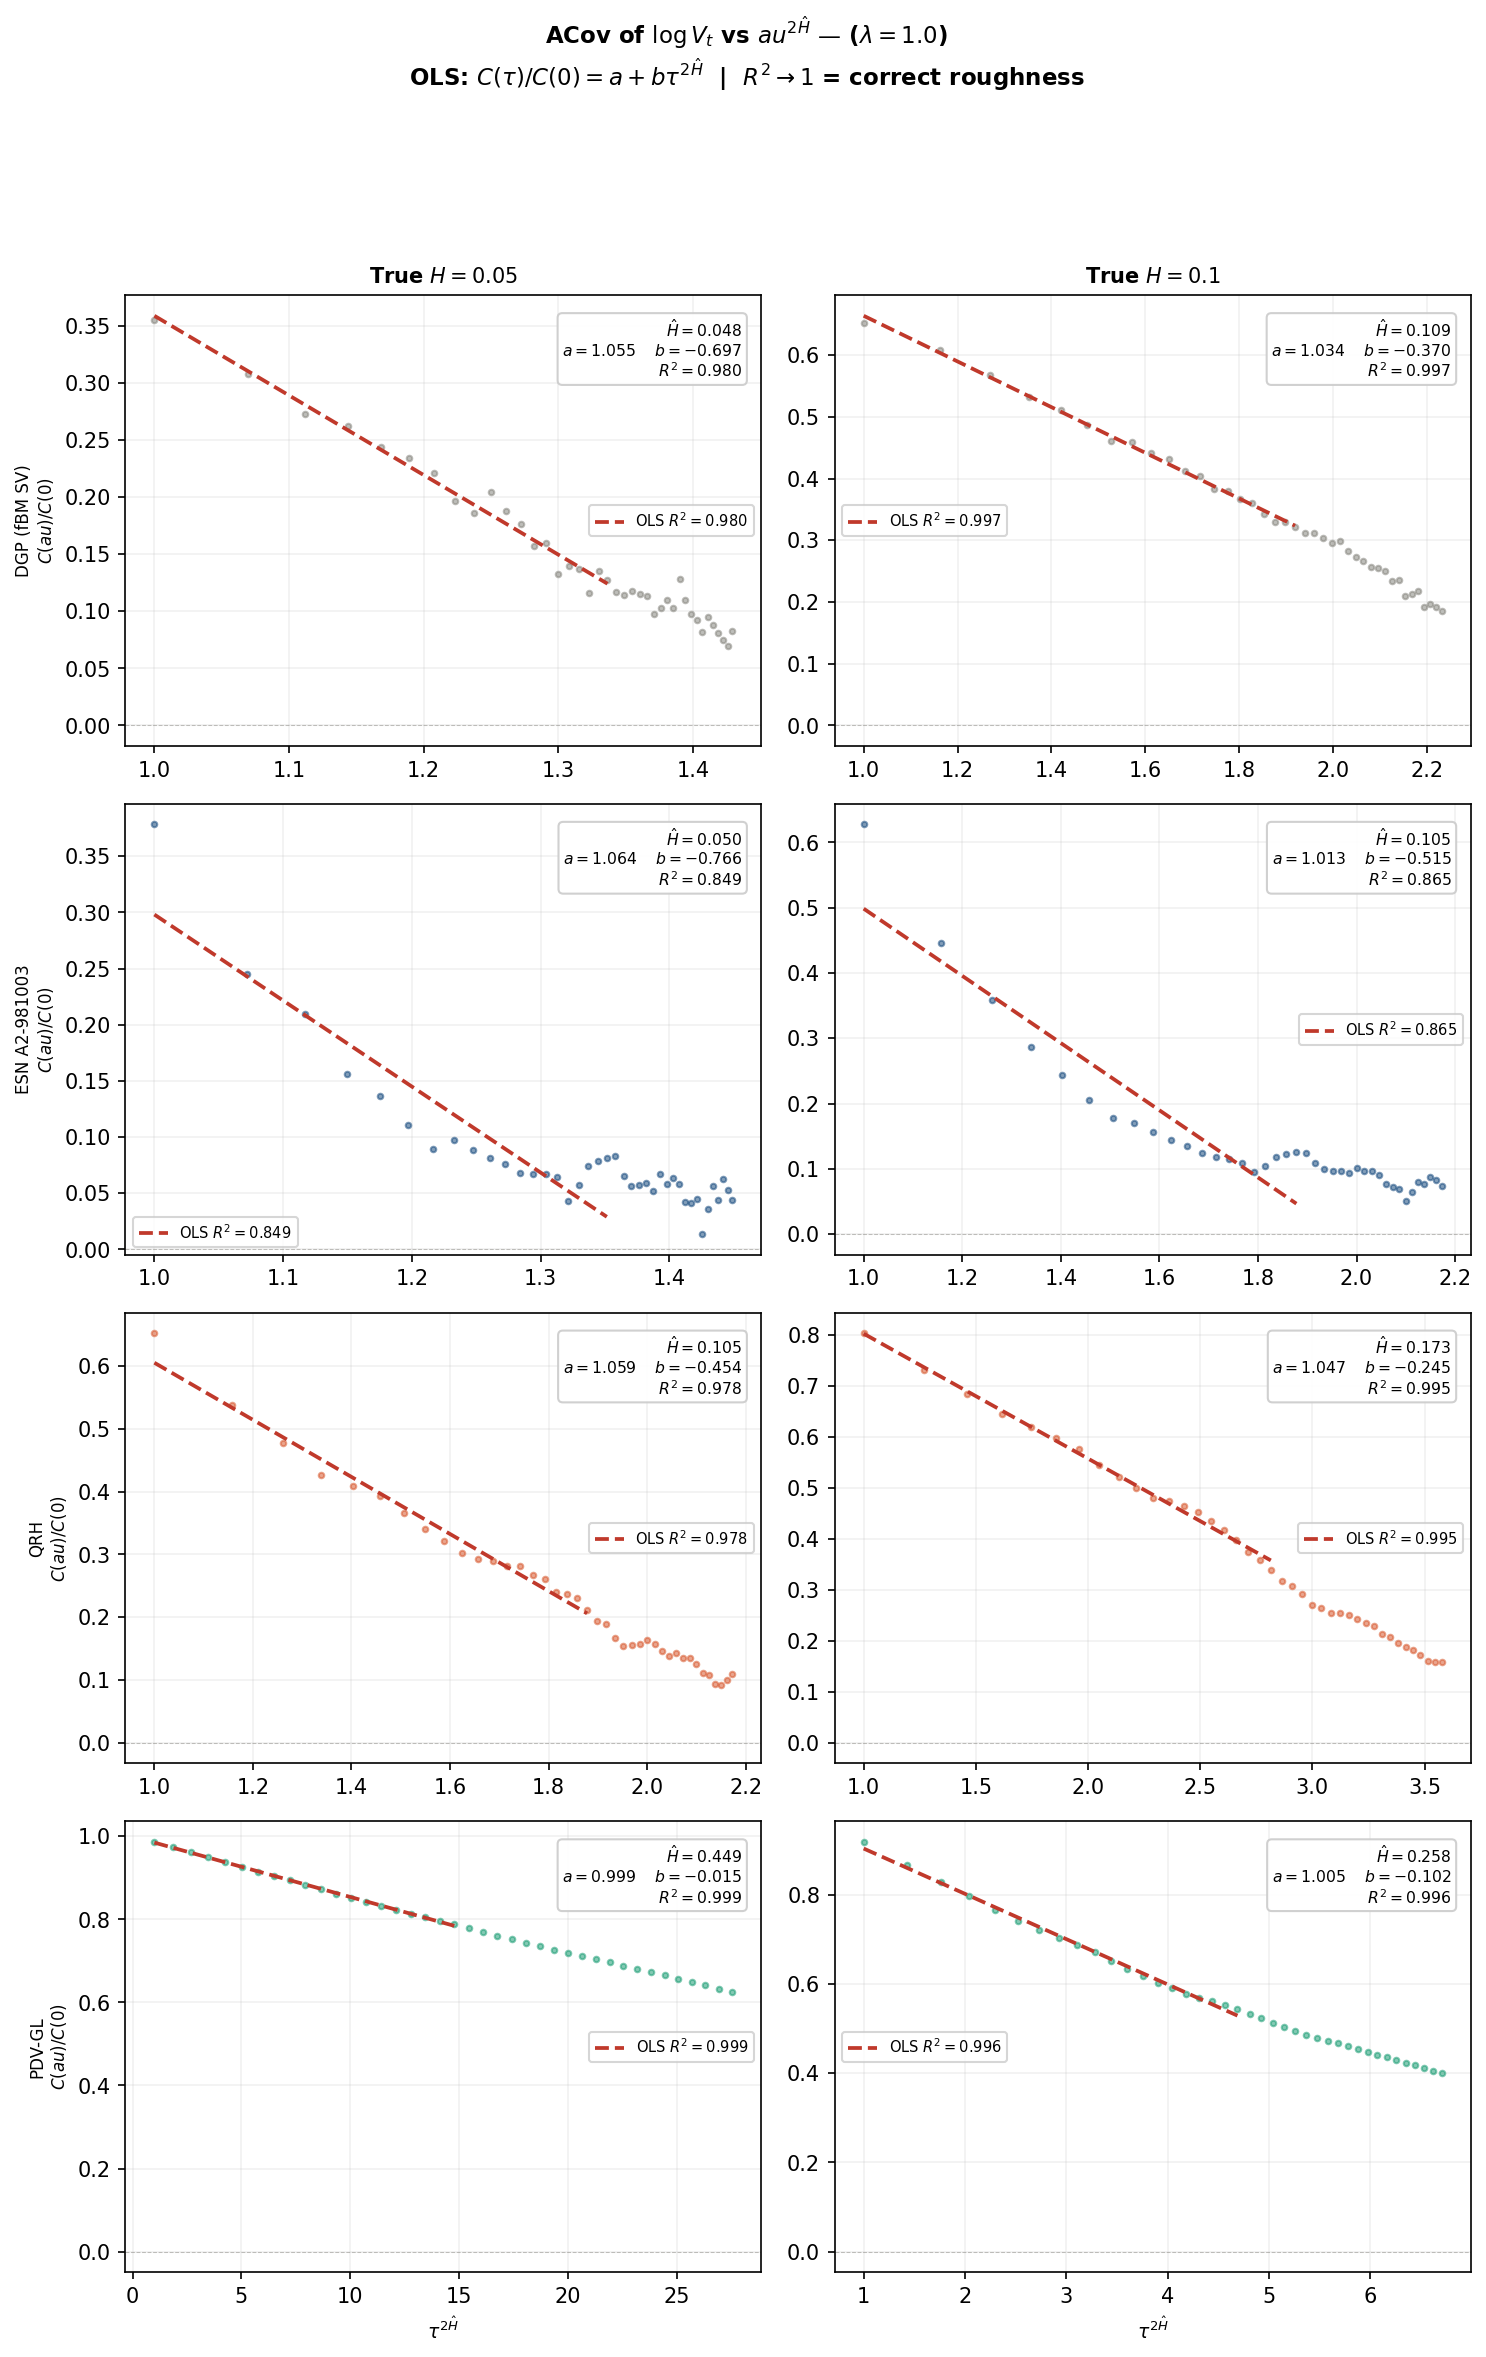
\includegraphics[width=0.95\textwidth]{roughness_h05_h10_out_acf_scaling_lam1p0.png}
\caption{Autocovariance of $\log V_t$ against $\tau^{2\hat H}$, per model (rows) and true $H\in\{0.05,0.10\}$ (columns), with the OLS fit and $R^2$ annotated in each panel.}
\label{fig:acov}
\end{figure}
\subsection{Diagnostic 3: Scale invariance}
$S_q(\tau)\sim\tau^{\zeta(q)}$; $H(q)=\zeta(q)/q$; $\mu(q)=\zeta(q)-q\zeta(1)$.
Monofractal DGP: all three are constant/zero.
\begin{figure}[H]
\centering
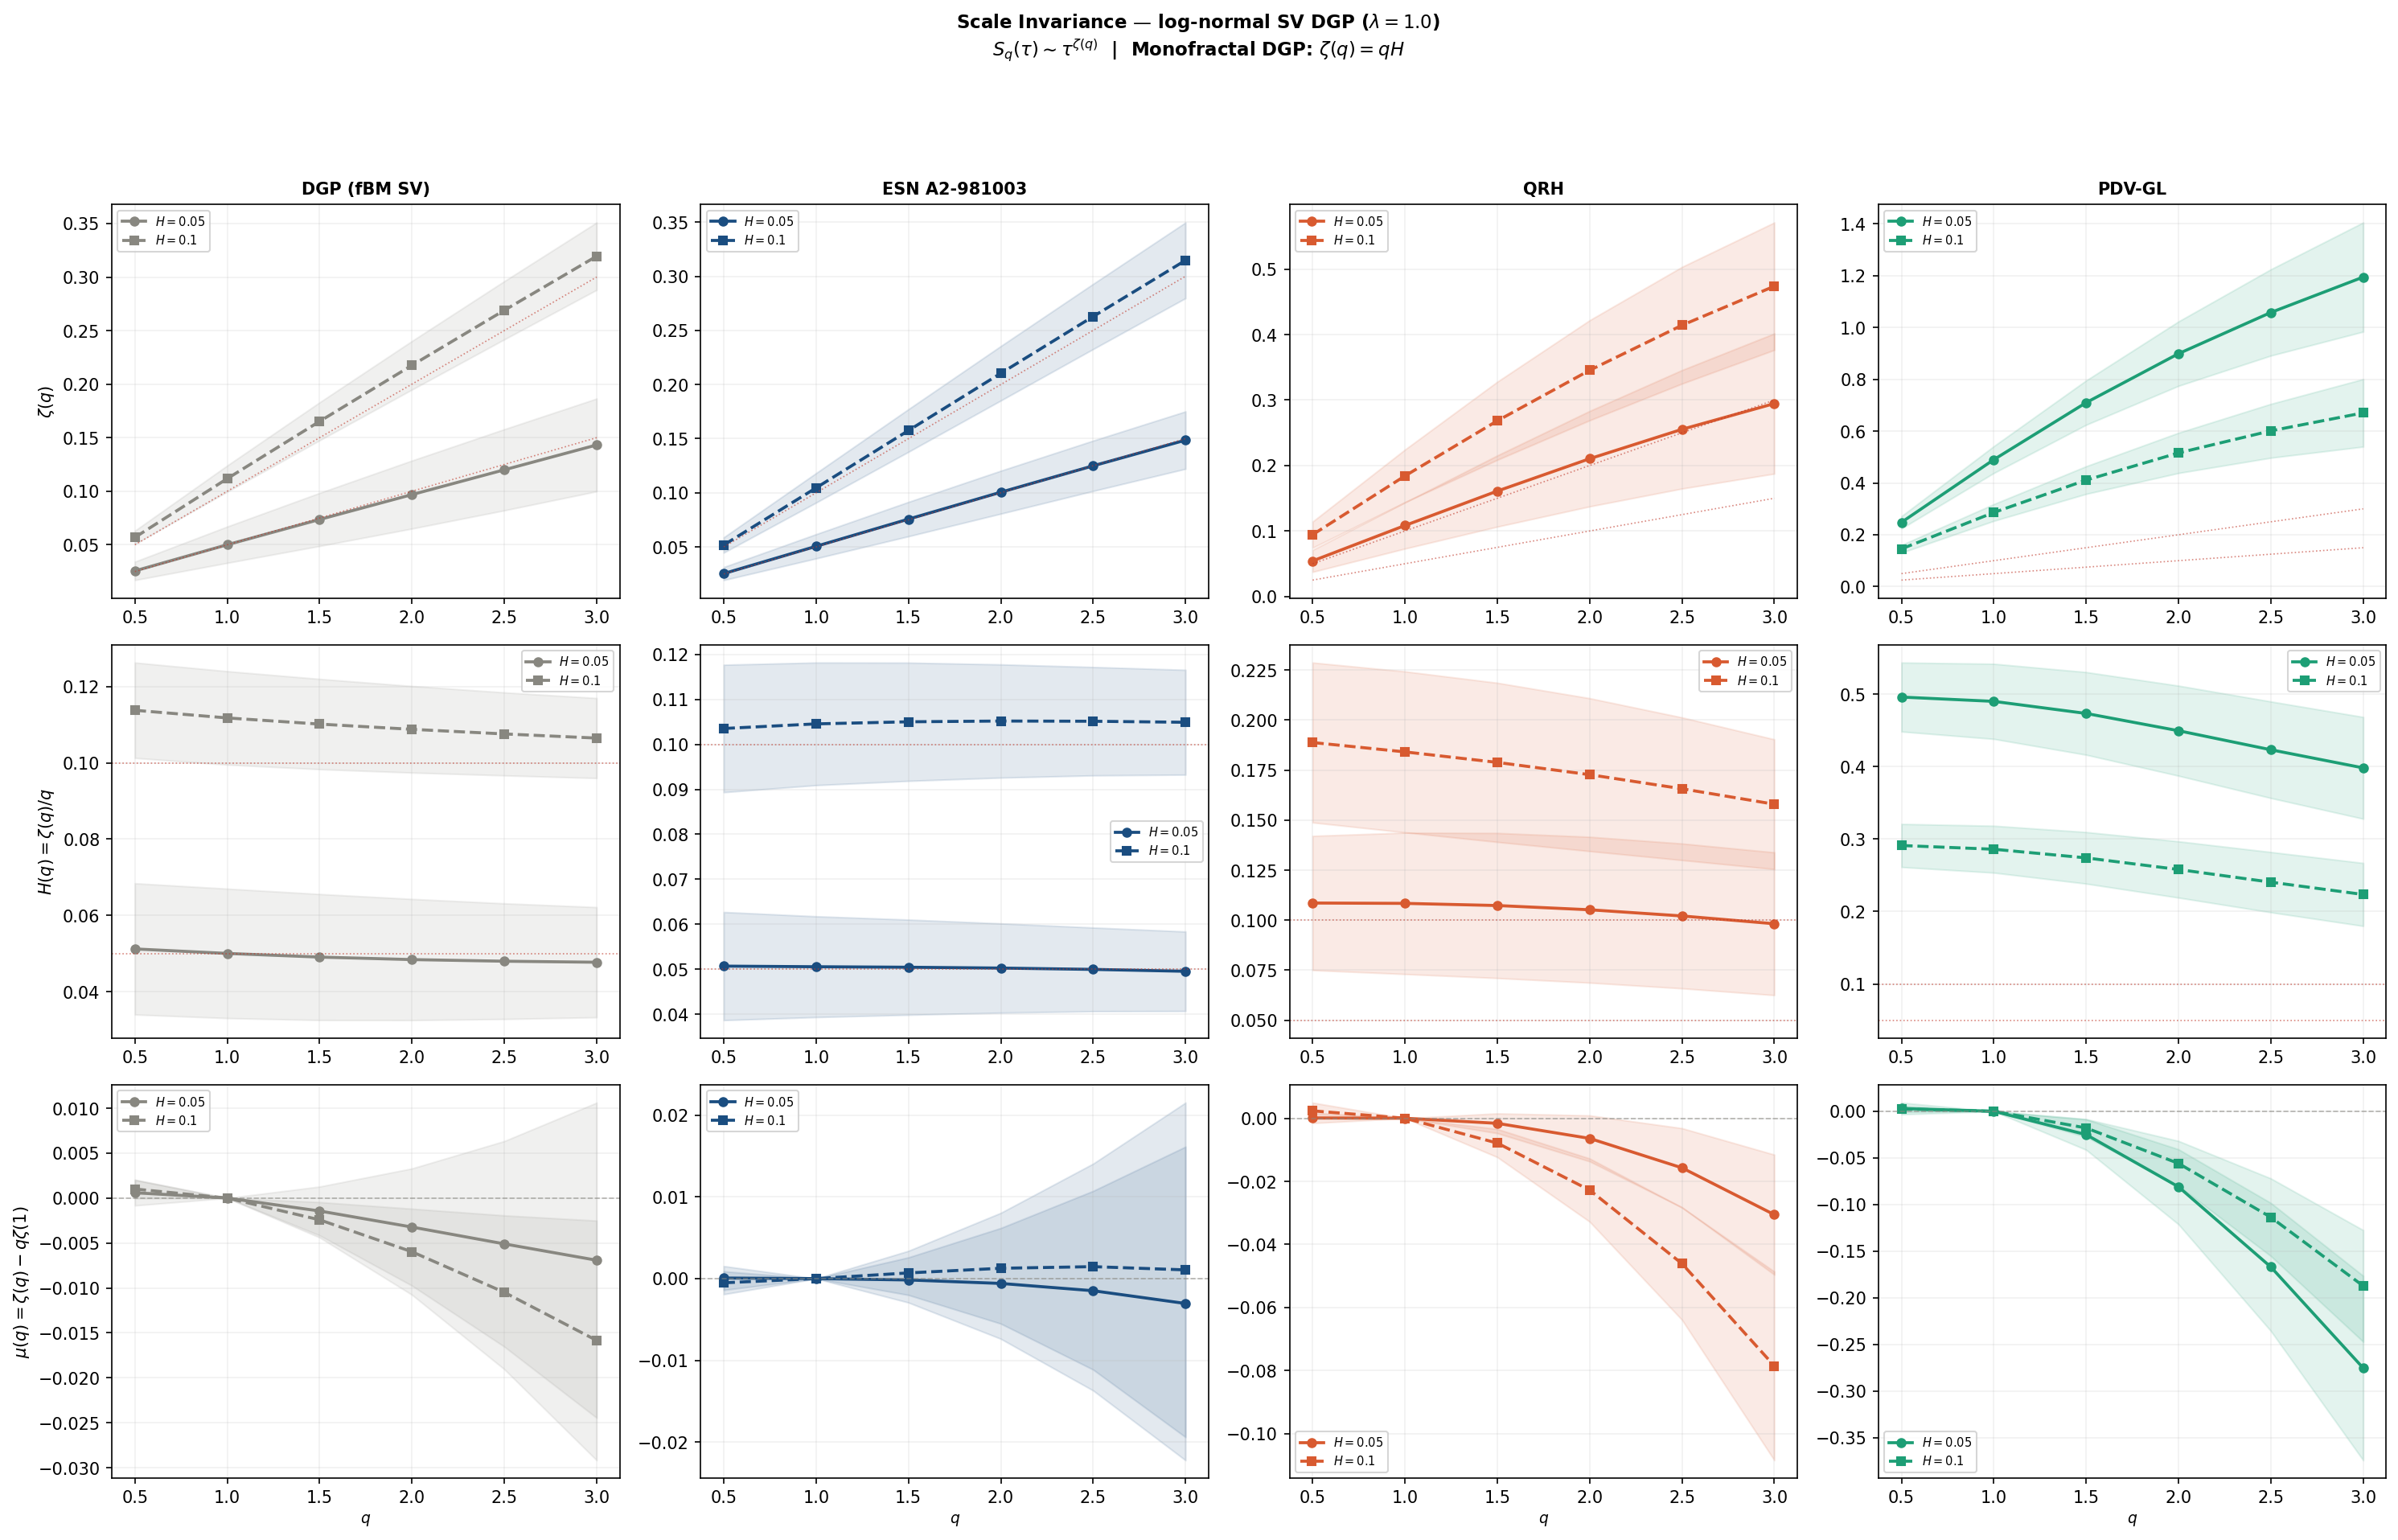
\includegraphics[width=0.95\textwidth]{roughness_h05_h10_out_scale_inv_lam1p0.png}
\caption{Scale invariance: structure-function exponent $\zeta(q)$ (top row), generalised Hurst function $H(q)=\zeta(q)/q$ (middle row), and multifractality measure $\mu(q)=\zeta(q)-q\zeta(1)$ (bottom row), per model (columns) and true $H\in\{0.05,0.10\}$ (line style). A flat $H(q)$ and $\mu(q)\equiv0$ indicate monofractal behaviour, matching the DGP.}
\label{fig:scaleinv}
\end{figure}
\section{Summary Figure}
Cross-diagnostic summary of $\hat H$ versus the true $H$, aggregating Diagnostic~1 across both $H$ values tested.
\begin{figure}[H]
\centering
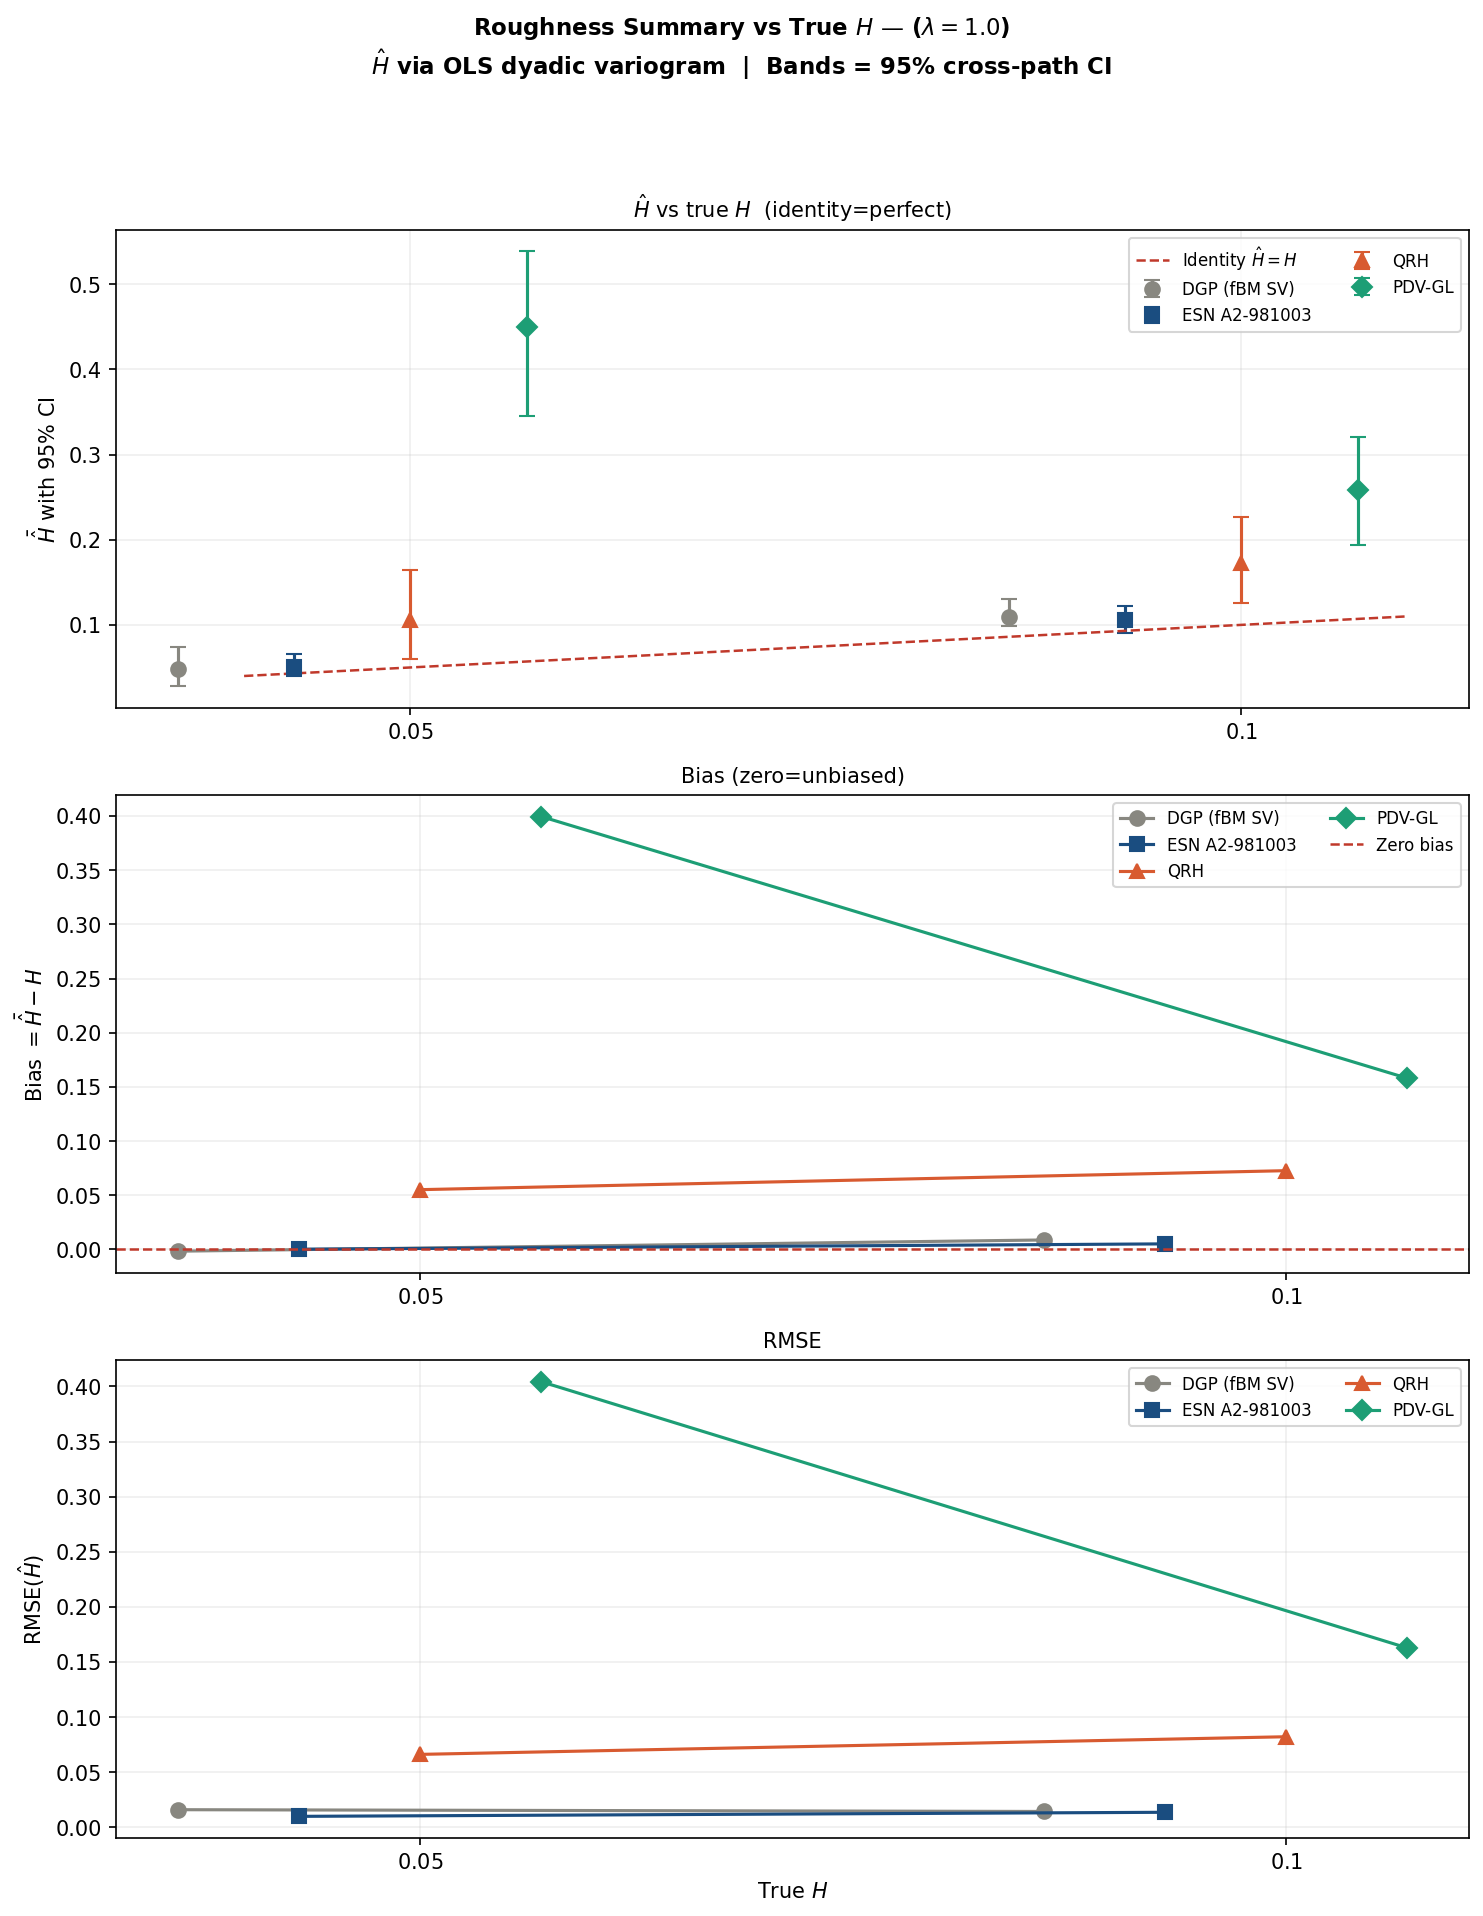
\includegraphics[width=0.85\textwidth]{roughness_h05_h10_out_hurst_summary_lam1p0.png}
\caption{$\hat H$ vs.\ true $H$ (top; identity line = perfect), bias (middle), and RMSE (bottom), per model, across both true $H$ values tested at $\lambda=1.0$.}
\label{fig:hurstsummary}
\end{figure}
\section{Monte Carlo Setup}
\begin{center}\renewcommand{\arraystretch}{1.4}
\begin{tabular}{ll}\toprule Parameter & Value \\\midrule
DGP paths & 30 \\ Cal.\ paths & 4 \\ Cal.\ days & 600 \\
Final paths & 30 \\ Final days & 2500 \\ Burn-in & 500 \\
$\Delta t$ & 1 (daily) \\ Dyadic lags & $\{1,2,4,8,16,32,64\}$ \\
Structure function $q$ & $\{0.5,1.0,1.5,2.0,2.5,3.0\}$ \\
ACov lags $\tau_{\max}$ & 20 \\
\bottomrule\end{tabular}\end{center}
\begin{thebibliography}{9}
\bibitem{gatheral2018} J.\ Gatheral, T.\ Jaisson, M.\ Rosenbaum.
\textit{Volatility is rough}. QF 18(6), 2018.
\bibitem{bourgey2026} F.\ Bourgey, J.\ Gatheral.
\textit{Quadratic Rough Heston}. SSRN:5239929, 2026.
\bibitem{guyon2023} J.\ Guyon, J.\ Lekeufack.
\textit{Volatility is (mostly) path-dependent}. QF 23(9), 2023.
\end{thebibliography}
\end{document}
